%%%%%%%%%%%%%%%%%%%%%%%%%%%%%%%%%%%%%%%%%%%%%%%%%%%%%%%%%%%%%%%%%
%2345678901234567890123456789012345678901234567890123456789012345
%        1         2         3         4         5         6     
\chapter{Economic model predictive control}
\label{cha:economic}

Static set-point tracking of the optimal leads to maximal crop growth in the greenhouse.
But such an implementation is neither market-driven nor efficient.

Since there is often a region of optimal parameters yet another MPC approach is presented. 
Assuming a region of optimal greenhouse temperature from \unit[24]{°C} to \unit[26]{°C}, operating the greenhouse at the lower bound requires less heating energy.
The quadratic objective function of conventional MPC is not able to involve this fact.

Furthermore, renewable energy sources, customer stimulus and many other effects produce regularly changing energy prices which are depicted in \cref{fig:electricity_tariff}.
The intraday of the electricity tariff was generated covering the major characteristics of the energy market.
From 0 a.m. to 4 a.m. when most people are asleep energy is the cheapest while in the early evening when people return from work energy is the most expensive.

\begin{figure}[t]
\begin{center}
	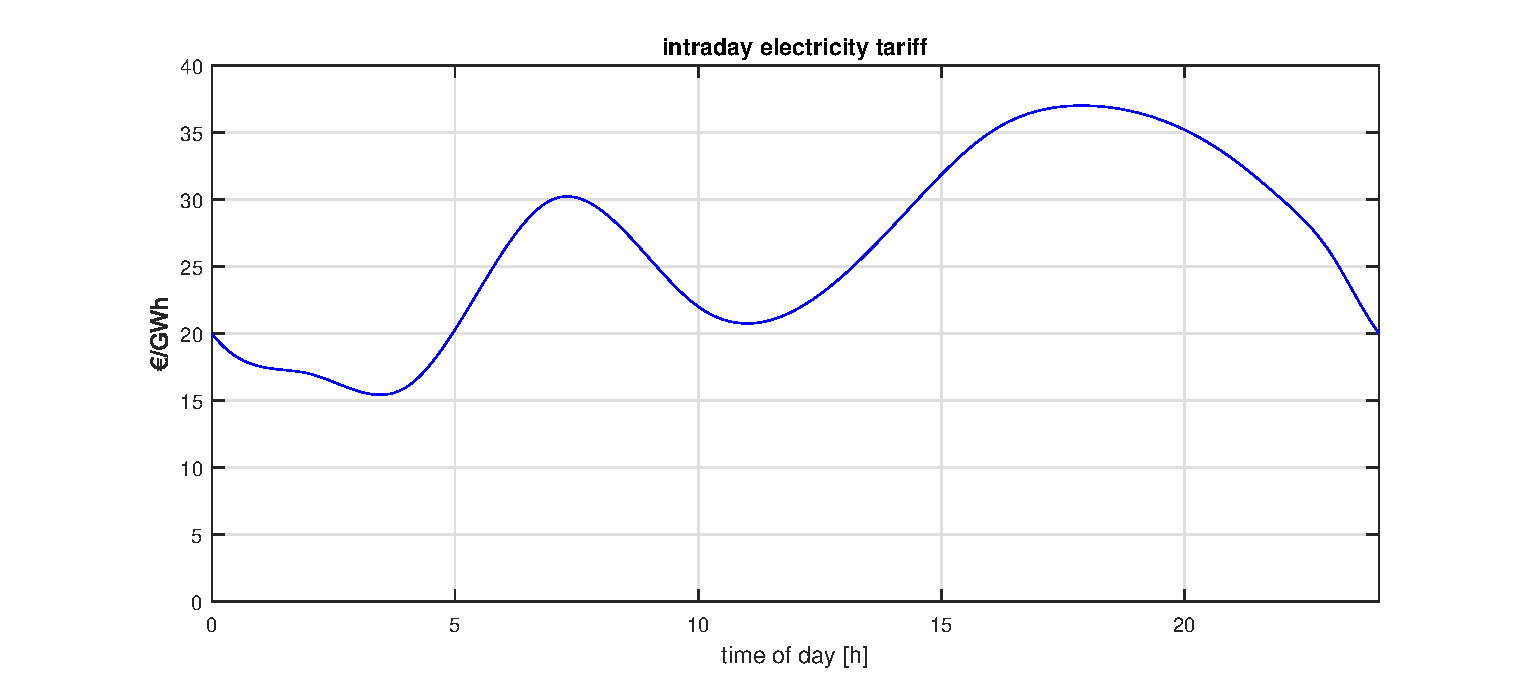
\includegraphics[width=\textwidth]{../Figures/intraday_electricity_tariff.eps}
	\caption{Intraday of the electricity tariff}
	\label{fig:electricity_tariff}
\end{center}
\end{figure}

One possibility to cope with the requirements of the modern energy market is economic model predictive control (EMPC).
An overview of approaches to economic process optimization is provided in \cite{Rawlings.2012}, \cite{Tran.2014} and \cite{Ellis.2016}.
First, the idea of EMPC is presented in \cref{sec:empcs}.
Then EMPC is applied to the operation of the greenhouse in \cref{sec:ecc}.
In \cref{sec:comp_sp_empc} the results of set-point tracking MPC and EMPC are compared using the augmented model predictive derived in \cref{sec:augmentedcontroller}.

%%%%%%%%%%%%%%%%%%%%%%%%%%%%%%%%%%%%%%%%%%%%%%%%%%%%%%%%%%%%%%%%%%%%%%%%%%%%%%%%%%%%%%%%%%%%%%%%%%%%%%%%%%%%%%%%%%%%%%%
%%%%%%%%%%%%%%%%%%%%%%%%%%%%%%%%%%%%%%%%%%%%%%%%%%%%%%%%%%%%%%%%%%%%%%%%%%%%%%%%%%%%%%%%%%%%%%%%%%%%%%%%%%%%%%%%%%%%%%%
%%%%%%%%%%%%%%%%%%%%%%%%%%%%%%%%%%%%%%%%%%%%%%%%%%%%%%%%%%%%%%%%%%%%%%%%%%%%%%%%%%%%%%%%%%%%%%%%%%%%%%%%%%%%%%%%%%%%%%%

\section{Preliminaries}
\label{sec:empcs}

EMPC is an off steady-state dynamic process optimization scheme.
Instead of tracking a set-point optimal regions and an economic objective function are defined.
The aim of EMPC is to optimize the economically efficient operation of a process by maximizing the profit or minimizing the costs.
Often the optimal point for operating the process with respect to the objective function is at the limits.

For the greenhouse the state constraints limit the region of parameters for optimal crop growth.
The state constraints are implemented as soft constraints.
Soft constraints avoid infeasibility for small violations of the limits.
Whereas the input constraints are hard constraints because they are physical limits of the actuators.
The constraints of the variables are summarized in \cref{tab:varconstraints}.

\begin{table}[htb]
	\centering
		\begin{tabular}{cccc}
		quantities                    &  lower bound     &  upper bound     &  unit                  \\\midrule
$X_{T,a}$        &  \unit[24]{}     &  \unit[26]{}     &  $\unit[]{^\circ C}$   \\
$X_{H_{a,a}}$    &  \unit[0.01]{}   &  \unit[0.02]{}   &  $\unit[]{kg/m^3}$     \\
$U_{ven}$        &  \unit[1]{}    &  \unit[100]{}    &  $\unit[]{\%}$         \\
$U_{shd}$        &  \unit[0]{}      &  \unit[0.7]{}    &  $\unit[]{-}$          \\
$U_{heat}$       &  \unit[0]{}      &  \unit[1000000]{}&  $\unit[]{W/m^2}$      \\
$U_{hum}$        &  \unit[0]{}      &  \unit[0.2]{}    &  $\unit[]{\nicefrac{kg}{m^5 \cdot s}}$   \\\bottomrule
\end{tabular}
	\caption{Constraints of the controlled variables $X_{(\cdot)}$ and manipulated variables $U_{(\cdot)}$.}
	\label{tab:varconstraints}
\end{table}

Since heating is the main cost for operating a greenhouse in the winter the objective function for EMPC is described by:
\begin{equation}\label{eq:J_eco}
J_{eco} = U_{heat} \cdot t_{step} \cdot p_{E} \cdot c_{area,ss} + p_{W} \cdot U_{hum},
\end{equation}
where $p_{E}$ is the current electricity tariff and $p_{W}$ is a penalty for water consumption.
Those possibly time-variable parameters are denoted as $\mathbf{d}_{eco}(t)$.
The first term gives the cost in $\unit[]{\text{\euro}}$ for each computation step.
The second term is added to minimize the water usage for humidification.

The description of EMPC is very similar to conventional MPC \eqref{eq:description_conventional_mpc} and to set-point tracking MPC \eqref{eq:setup_setpoint}.
The economic optimal control problem is fully described by:
\begin{subequations}\label{eq:setup_empc}
\begin{align}
\min \int_0^{t_f} \!  &J_{eco}(\mathbf{x}(t),\mathbf{u}(t);\mathbf{d}_{eco}(t)) \, \mathrm{d}t
\end{align}
subject to:
\begin{align}
\dot{\mathbf{x}}_{pm}(t) &= f(\mathbf{x}(t),\mathbf{u}(t);\mathbf{d}(t)),\\
\mathbf{x}(t) &\in \mathcal{X}, \, \mathbf{u}(t)  \in \mathcal{U}.
\end{align}
\end{subequations}

In the following two sections three different MPC approaches are compared.
The differences between the approaches and their denomination is given in \cref{tab:nomenclature_MPC}.

\begin{figure}[t]
\begin{center}
	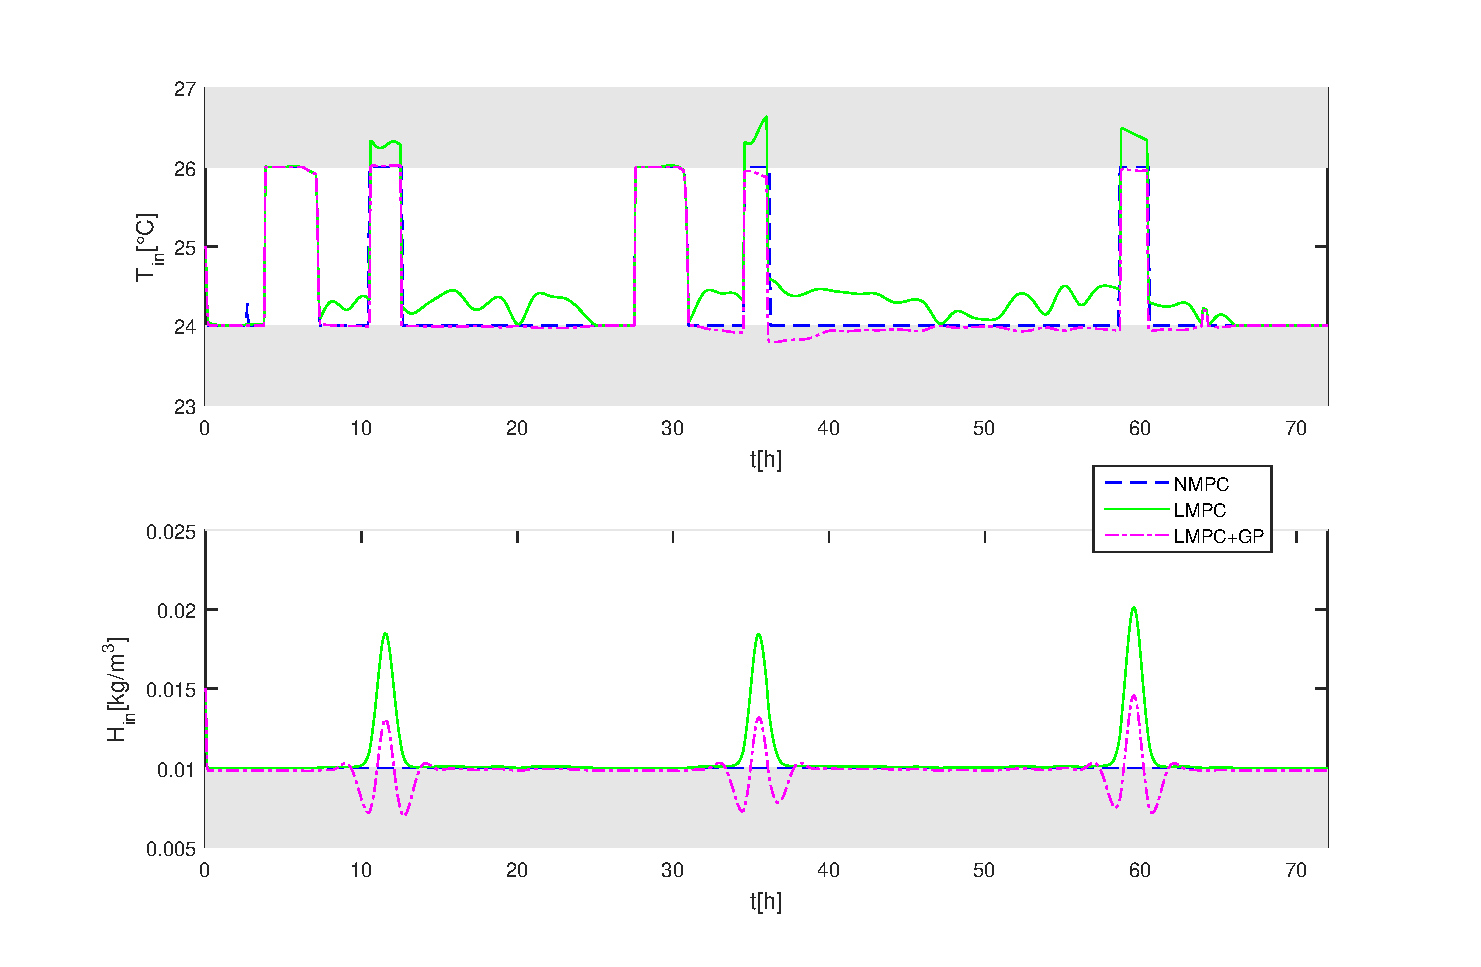
\includegraphics[width=\textwidth]{../Figures/economic_states.eps}
	\caption{State trajectories of EMPC}
	\label{fig:economic_states}
\end{center}
\end{figure}

%%%%%%%%%%%%%%%%%%%%%%%%%%%%%%%%%%%%%%%%%%%%%%%%%%%%%%%%%%%%%%%%%%%%%%%%%%%%%%%%%%%%%%%%%%%%%%%%%%%%%%%%%%%%%%%%%%%%%%%
%%%%%%%%%%%%%%%%%%%%%%%%%%%%%%%%%%%%%%%%%%%%%%%%%%%%%%%%%%%%%%%%%%%%%%%%%%%%%%%%%%%%%%%%%%%%%%%%%%%%%%%%%%%%%%%%%%%%%%%
%%%%%%%%%%%%%%%%%%%%%%%%%%%%%%%%%%%%%%%%%%%%%%%%%%%%%%%%%%%%%%%%%%%%%%%%%%%%%%%%%%%%%%%%%%%%%%%%%%%%%%%%%%%%%%%%%%%%%%%

\section{Economic climate control}
\label{sec:ecc}

For the analysis of EMPC the same scenario was used as for set-point tracking (\cref{fig:disturbances_mpc}).
The figures were limited to 72 hours due to better visualisation.
NMPC was used as the benchmark since it includes a perfect prediction model.\par\medskip

\cref{fig:economic_states} shows that LMPC+GP enhances the quality of EMPC compared to LMPC.
The temperature trajectory of LMPC+GP stays mostly close to the one of NMPC while LMPC is often deviated.
Thus, the root mean square error for the temperature could be reduced by \unit[47]{\%}.
This results in a reduction of costs for operating the greenhouse by \unit[1.5]{\%} while providing better crop growth.

\begin{figure}[t]
	\begin{subfigure}[t]{0.49\textwidth}
		\includegraphics[width=\textwidth]{../Figures/economic_heating_electricity.eps}
		\caption{Electricity tariff}
		\label{fig:eco_heat_elec}
	\end{subfigure}
	\hfill
	\begin{subfigure}[t]{0.49\textwidth}
		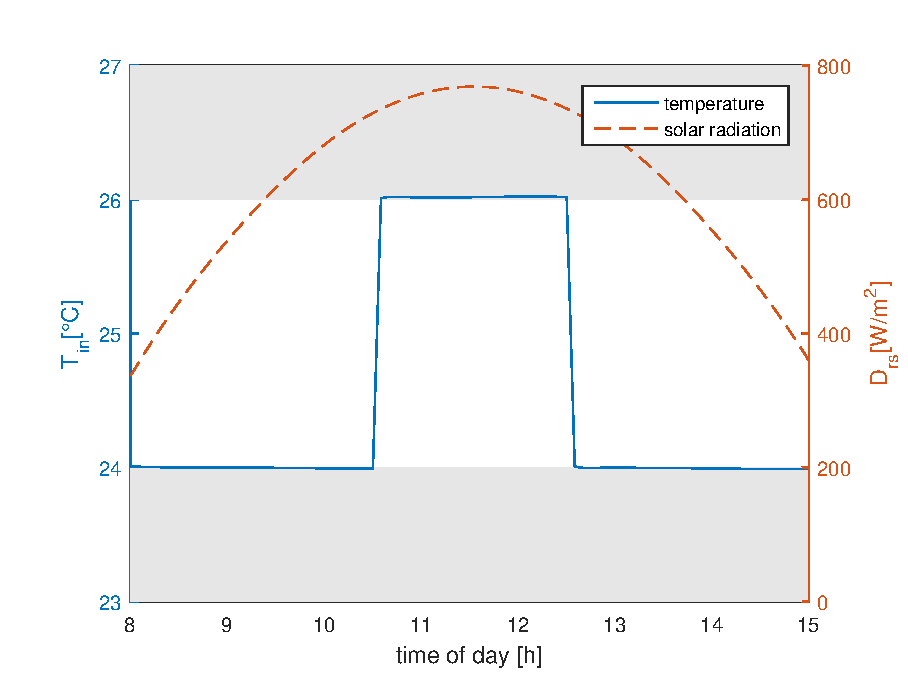
\includegraphics[width=\textwidth]{../Figures/economic_temperature_solar.eps}
		\caption{Solar radiation}
		\label{fig:eco_temp_sol}
	\end{subfigure}
\caption{Effect of external variables on EMPC with LMPC+GP}
\label{fig:cons_dist}
\end{figure}

In most of the cases there are two peaks for the air temperature within every 24 hours where the temperature is driven to the upper bound.
Those peaks are due to capitalizing the influences of time-varying parameters and disturbances.
In those situations the air serves as a storage for cheap energy.

The first peak of the day is dedicated to more heating due to low energy prices.
The left pane of \cref{fig:cons_dist} shows this relation in detail.
When the price for energy is the lowest ($t \leq \unit[4]{h}$) the heating reaches its highest values.
Throughout the day the heating is significantly lower since the energy is more expensive.

The second peak is dedicated to the gratuitous energy delivered by the sun.
Around noon when the solar radiation reaches its peak the air temperature inside the greenhouse rises to the upper bound.
This effect is depicted on the right pane of \cref{fig:cons_dist}.

The left pane of \cref{fig:detail_state_traj} shows a detail of the  temperature trajectory around noon ($t = \unit[84]{h}$).
Due to underestimating the impact of the solar radiation LMPC is deviated by trend to higher temperatures.
This leads to violations of the upper bound.
Due to the GPs LMPC+GP is able to estimate the nonlinear effect of the solar radiation.
Therefore, the maximum violations of the temperature constraints could be reduced by \unit[63]{\%}.\par\medskip

\begin{figure}[t]
	\begin{subfigure}[t]{0.49\textwidth}
		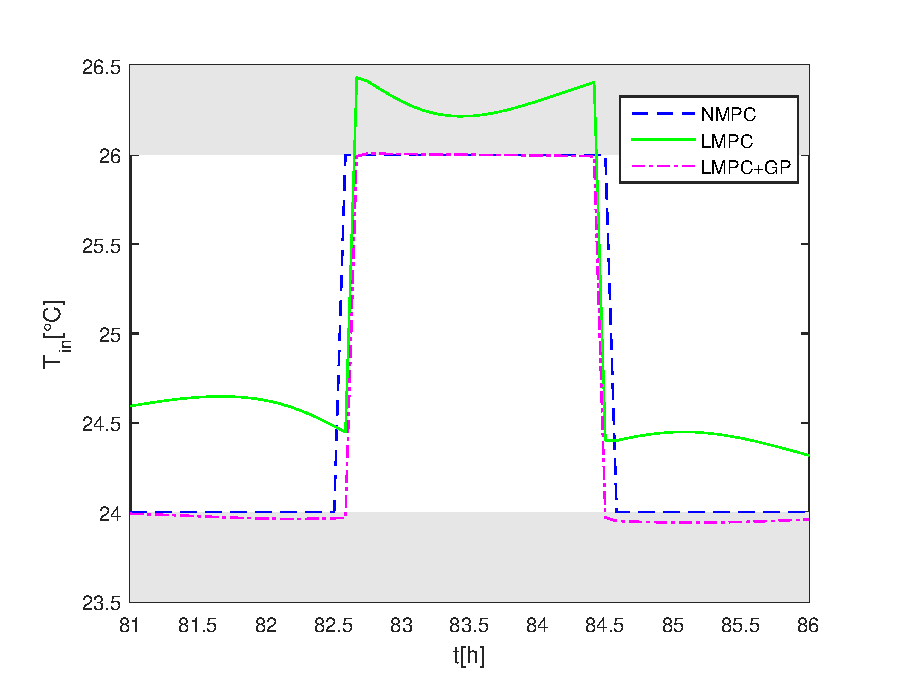
\includegraphics[width=\textwidth]{../Figures/economic_detail_temperature.eps}
		\caption{Temperature}
		\label{fig:eco_det_temp}
	\end{subfigure}
	\hfill
	\begin{subfigure}[t]{0.49\textwidth}
		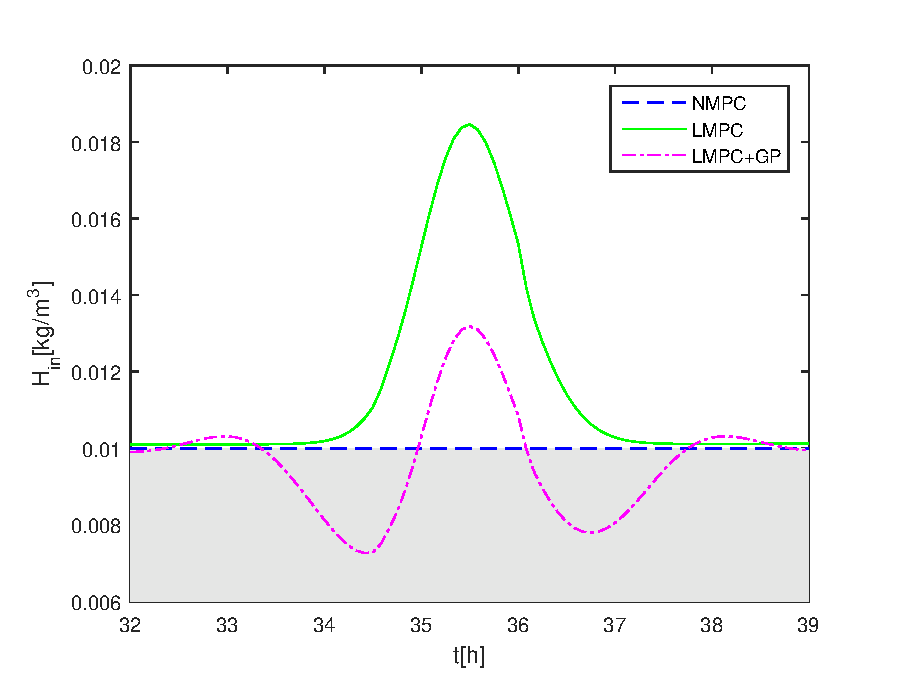
\includegraphics[width=\textwidth]{../Figures/economic_detail_humidity.eps}
		\caption{Humidity}
		\label{fig:eco_det_hum}
	\end{subfigure}
\caption{Details of the state trajectories}
\label{fig:detail_state_traj}
\end{figure}

The humidity trajectories are depicted in \cref{fig:economic_states}.
Since the humidification system is the main source for the inside air humidity, operating the system at the lower bound minimizes the water usage.
The solar radiation is the main influence for the crop transpiration.
Since the effect is nonlinear the control of LMPC and LMPC+GP gets worse the bigger the solar radiation becomes.
The right pane of \cref{fig:detail_state_traj} shows the humidity trajectories from 8 a.m. to 3 p.m. in detail.
LMPC+GP stays closer to the to optimal trajectory of NMPC than LMPC.
The GPs enable LMPC+GP to compensate the nonlinear effect while LMPC gets heavily deviated.
Hence, the root mean square error of LMPC+GP is reduced by \unit[43]{\%} compared to LMPC.
The violations of the lower bound by LMPC+GP are not critical since the correct temperature is more important for crop growth.\par\medskip

The input trajectories are presented in \cref{fig:economic_control}.
For all three MPC approaches the trajectories are very similar.
The inputs do not reach their upper limits and their progress is smooth.
This means both linear prediction models compute reasonable control.

The input trajectories of ventilation $U_{ven}$ and the shades $U_{shd}$ exhibit several flat areas.
Both manipulated variables are bilinearly related with disturbance variables.
The effect of the bilinearity was explained using the example of \eqref{eq:simple_rs}.
When the disturbances are zero the inputs have no impact.
Thus, they are set to the middle of their physical limits.

\begin{figure}[t]
\begin{center}
	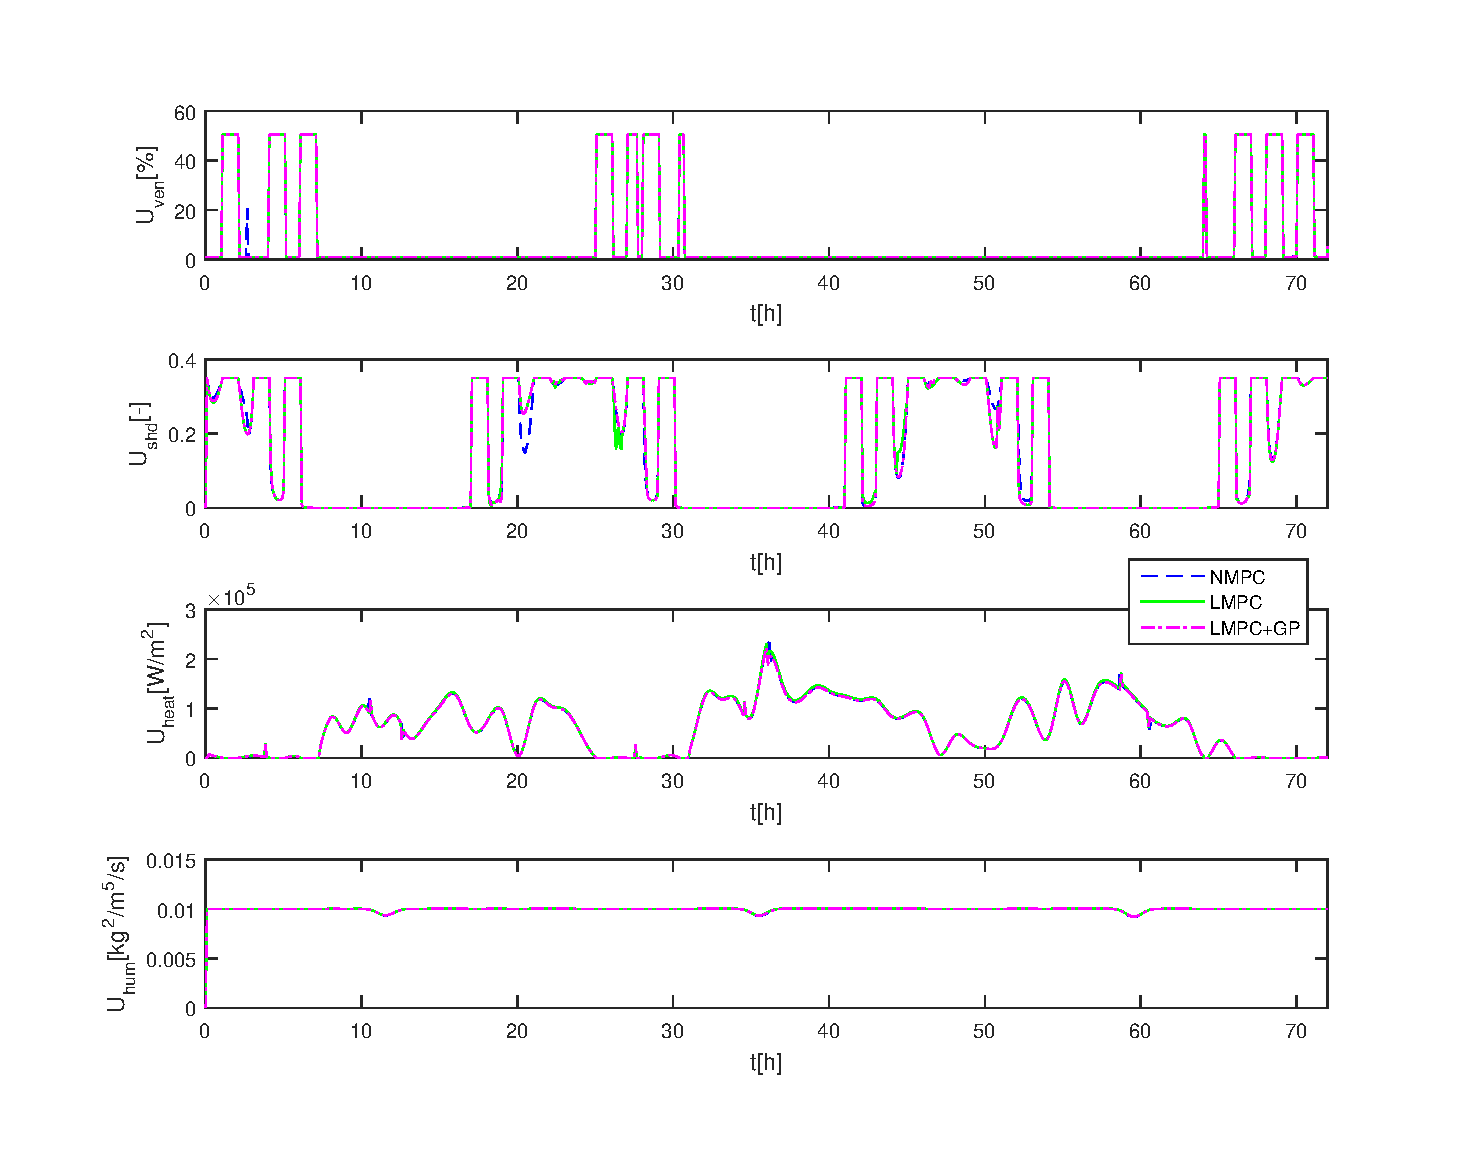
\includegraphics[width=\textwidth]{../Figures/economic_control.eps}
	\caption{Input trajectories of EMPC}
	\label{fig:economic_control}
\end{center}
\end{figure}

\begin{table}[htb]
	\centering
		\begin{tabular}{ccccc}
		\multicolumn{2}{c}{quantities}                             &    NMPC    &    LMPC    &    LMPC+GP           \\\midrule
		maximum      & temp. $[\unit{^\circ C}]$          &      -     &    $0.60$  &     $0.22$           \\\cline{2-5}
		violation    & hum. $[\unitfrac{kg}{m^3}]$        &      -     &      -     & $2.84 \cdot 10^{-3}$ \\\midrule
		root mean    & temp. $[\unit{^\circ C}]$          &      -     &   $0.2815$ &   $0.1486$           \\\cline{2-5}
		square error & hum. $[\unitfrac{kg}{m^3}]$        &      -     &   $0.0024$ &    $0.0014$          \\\midrule
		\multirow{3}{*}{mean} & $U_{heat}$ $[\unitfrac{W}{m^2}]$ & $5.619 \cdot 10^{4}$ & $5.705 \cdot 10^{4}$ & $5.605 \cdot 10^{4}$ \\\cline{2-5}
		                      & $U_{hum}$ $[\unitfrac{kg^2}{m^5 \cdot s}]$ & $0.01$ & $0.01$ & $0.01$ \\\cline{2-5}
		& cost $[\unitfrac{\text{\euro}}{h}]$  & $109.35$ & $111.04$ & $109.09$ \\\bottomrule
		\end{tabular}
		\vspace{1mm}
	\caption{Comparison of the EMPC schemes}
	\label{tab:analysis_empc}
\end{table}

%%%%%%%%%%%%%%%%%%%%%%%%%%%%%%%%%%%%%%%%%%%%%%%%%%%%%%%%%%%%%%%%%%%%%%%%%%%%%%%%%%%%%%%%%%%%%%%%%%%%%%%%%%%%%%%%%%%%%%%
%%%%%%%%%%%%%%%%%%%%%%%%%%%%%%%%%%%%%%%%%%%%%%%%%%%%%%%%%%%%%%%%%%%%%%%%%%%%%%%%%%%%%%%%%%%%%%%%%%%%%%%%%%%%%%%%%%%%%%%
%%%%%%%%%%%%%%%%%%%%%%%%%%%%%%%%%%%%%%%%%%%%%%%%%%%%%%%%%%%%%%%%%%%%%%%%%%%%%%%%%%%%%%%%%%%%%%%%%%%%%%%%%%%%%%%%%%%%%%%

\section{Comparison of set-point tracking MPC and EMPC}
\label{sec:comp_sp_empc}

The definitions of set-point tracking MPC \eqref{eq:setup_setpoint} and EMPC \eqref{eq:setup_empc} are very similar.
However, the choice of the objective function and the state constraints have a huge impact on the performance of MPC.
For the analysis in this section exclusively the expanded MPC scheme (LMPC+GP) was used.


\begin{figure}[t]
\begin{center}
	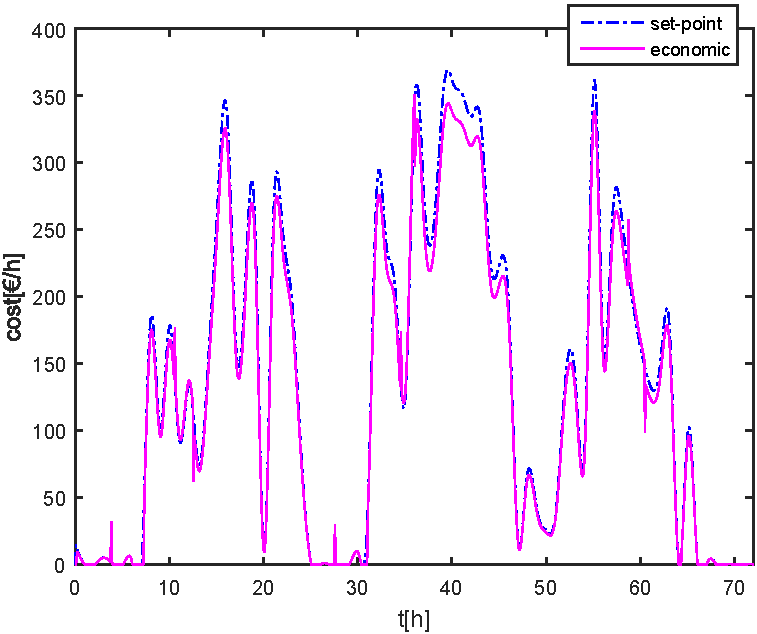
\includegraphics[width=\textwidth]{../Figures/cost_big.pdf}
		\caption{Progress of the operating cost}
		\label{fig:cost_progress}
\end{center}
\end{figure}

\cref{tab:analysis_versus} shows the operating effort of the greenhouse using the control strategies presented \cref{cha:setpoint} and \cref{cha:economic}.
Applying EMPC leads to significant savings concerning operating costs compared to set-point tracking MPC, as \cref{fig:cost_progress}shows.

\begin{table}[b]
	\centering
		\begin{tabular}{ccccc}
		\multicolumn{1}{c}{quantities}    &    unit                            &    set-point tracking     &        economic         &     savings             \\\midrule
		mean $U_{heat}$          & $[\unitfrac{W}{m^2}]$              &    $5.9205 \cdot 10^4$    &  $5.6051 \cdot 10^4$    &     $\unit[5.32]{\%}$   \\
		mean $U_{hum}$           & $[\unitfrac{kg^2}{m^5 \cdot s}]$   &   $99.731 \cdot 10^{-3}$  &  $99.561 \cdot 10^{-3}$ &     $\unit[0.15]{\%}$   \\
		mean cost                & $[\unitfrac{\text{\euro}}{h}]$     &          $115.50$         &        $109.09$         &     $\unit[5.54]{\%}$   \\\bottomrule
		\end{tabular}
		\vspace{1mm}
	\caption{Comparison of operating effort of the greenhouse}
	\label{tab:analysis_versus}
\end{table}

Due to the consideration of the intraday of the electricity tariff the cost was diminished by \unit[5.54]{\%}.
This means every hour more than \unit[6]{\euro} can be saved on average.
The energy used for heating the greenhouse was decreased by \unit[5.32]{\%}.
Also the consumption of water for humidification could be slightly reduced by \unit[0.15]{\%}.
\cref{fig:sp_vs_eco} illustrates the savings more detailed.
On the left the progress of the cost and on the right the progress of the humidification is depicted.\par\medskip

\begin{figure}[t]
	\begin{subfigure}[t]{0.49\textwidth}
		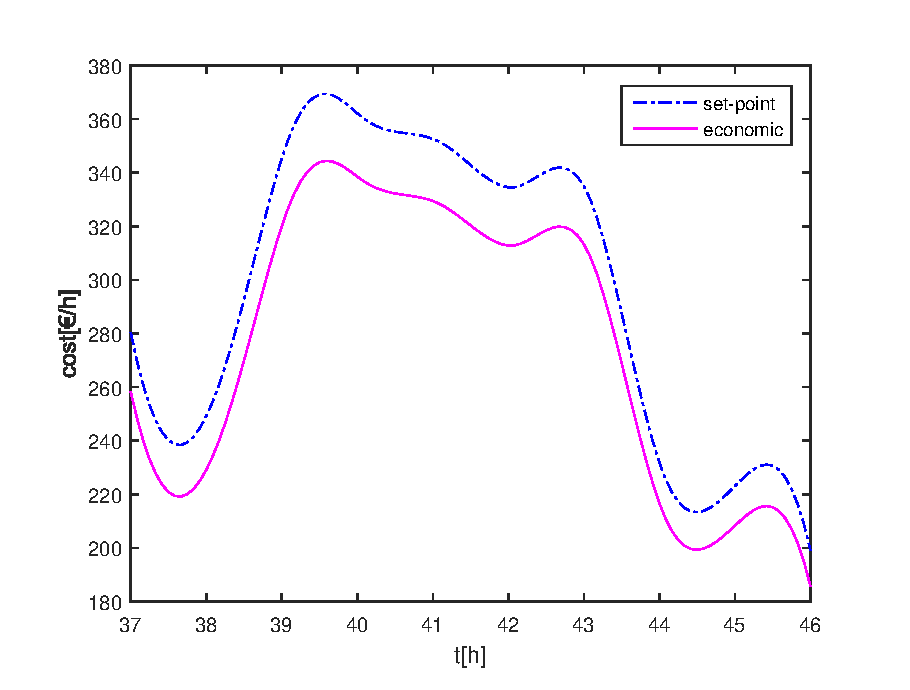
\includegraphics[width=\textwidth]{../Figures/economic_vs_setpoint_cost.eps}
		\caption{Operating cost}
		\label{fig:versus_cost}
	\end{subfigure}
	\hfill
	\begin{subfigure}[t]{0.49\textwidth}
		\includegraphics[width=\textwidth]{../Figures/economic_vs_setpoint_hum.eps}
		\caption{Humidification}
		\label{fig:versus_hum}
	\end{subfigure}
\caption{Detailed comparison of the operating effort}
\label{fig:sp_vs_eco}
\end{figure}

In the current chapter the control strategy EMPC was presented.
First EMPC was derived and stated.
Afterwards, it was shown that LMPC+GP performs better than LMPC and similar to NMPC applied to EMPC.
The current section presented the profit EMPC compared to set-point tracking MPC using LMPC+GP as the prediction model.
In the concluding chapter the outcomes of this work are summarized and reviewed.
Furthermore, directions for future works are provided.